\documentclass{article}

\usepackage[utf8]{inputenc}
\usepackage[MeX]{polski}
\usepackage{graphicx}   %do rysunków
\usepackage{wrapfig}    %do rysunków otoczonych tekstem
\usepackage{color}      %do użycia podst. kolorów oraz zdefiniowanych kolorów 
%do kolorowych referencji do rysunków, cytowań:
\usepackage{multirow}
\usepackage{longtable}
\usepackage{float}
\usepackage{indentfirst}
\usepackage[shortlabels]{enumitem}
\usepackage[colorlinks=true,linkcolor=blue,citecolor=green]{hyperref}

%do kolorowych referencji do rysunków, cytowań:
\usepackage{multicol}
\usepackage{colortbl}


%do pdfow
\usepackage{pdfpages}

\textwidth=16cm
\textheight=23cm
\topmargin=-2cm
\oddsidemargin=0cm

\title{}
\author{ }
\date{}

\begin{document}

\begin{table}[h!]
\centering
\begin{tabular}{|p{2.1cm}|p{2.1cm}|p{2.1cm}|p{2.1cm}|p{2.1cm}|p{2.1cm}|}\hline
\multicolumn{2}{|c|}{\textbf{Wstęp do fizyki ciała stałego}}
& \multicolumn{4}{c|}{\textbf{Projekt 2, zestaw 1}} \\ \hline
\multicolumn{2}{|l|}{Konrad Marciniak} & e-mail:
& \multicolumn{3}{c|}{konrad.marciniak.stud@pw.edu.pl}
\\ \hline
data:& & nr indeksu: & 311730 & grupa: & W2 \\ \hline
\multicolumn{6}{|c|}{\begin{tabular}[c]{@{}c@{}}Oświadczam, że jestem jedynym autorem/jedyną
autorką niniejszego projektu.\\Jestem świadomy/świadoma odpowiedzialności w przypadku podania fałszywej informacji.\\ \\ (podpis studenta)\end{tabular}} \\ \hline
\end{tabular}
\end{table}

\section*{Zadanie 1 - fonony}
Na podstawie mojego nr indeksu i poniższego równania został wylosowany zestaw nr 1.
$$ (\mbox{indeks mod 5}) + 1 = 1 $$

\begin{table}[ht!]
\centering
\begin{tabular}{|cccc|}
\hline
\multicolumn{4}{|c|}{Zestaw 1}                                                                                                    \\ \hline
\multicolumn{1}{|c|}{$M_1$} & \multicolumn{1}{c|}{$M_2$} & \multicolumn{1}{c|}{$\gamma_1$} & $\gamma_2$ \\ \hline
\multicolumn{1}{|c|}{4}    & \multicolumn{1}{c|}{1}    & \multicolumn{1}{c|}{2}                        & 3                        \\ \hline
\end{tabular}
\end{table}

Na następnej stronie przedstawione są obliczenia potrzebne do wyznaczenia zależności dyspersyjnej $\omega(q)$ dla fali fononów propagującęj się w jednowymiarowym, dwuatomowym łańcuchu periodycznym.

Otrzymane gałęzie fononowe:

\begin{itemize}
	\item Gałąź optyczna
		$$ \omega = \sqrt{ \frac{\sqrt{192 cos(qa) + 433}}{8} + \frac{25}{8} } $$
	\item Gałąź akustyczna
		$$ \omega = \sqrt{ - \frac{\sqrt{192 cos(qa) + 433}}{8} + \frac{25}{8} } $$
\end{itemize}

\renewcommand{\figurename}{Wykres}
\begin{figure}[ht!]
    \centering
    \includegraphics[width=0.7\textwidth]{./out/phonons.jpg}
    \caption{przedstawia wyżej wyznaczone gałęzie dla pierwszej strefy Brillouina $q\in(\frac{-\pi}{a};\frac{\pi}{a})$}
    \centering
\end{figure}

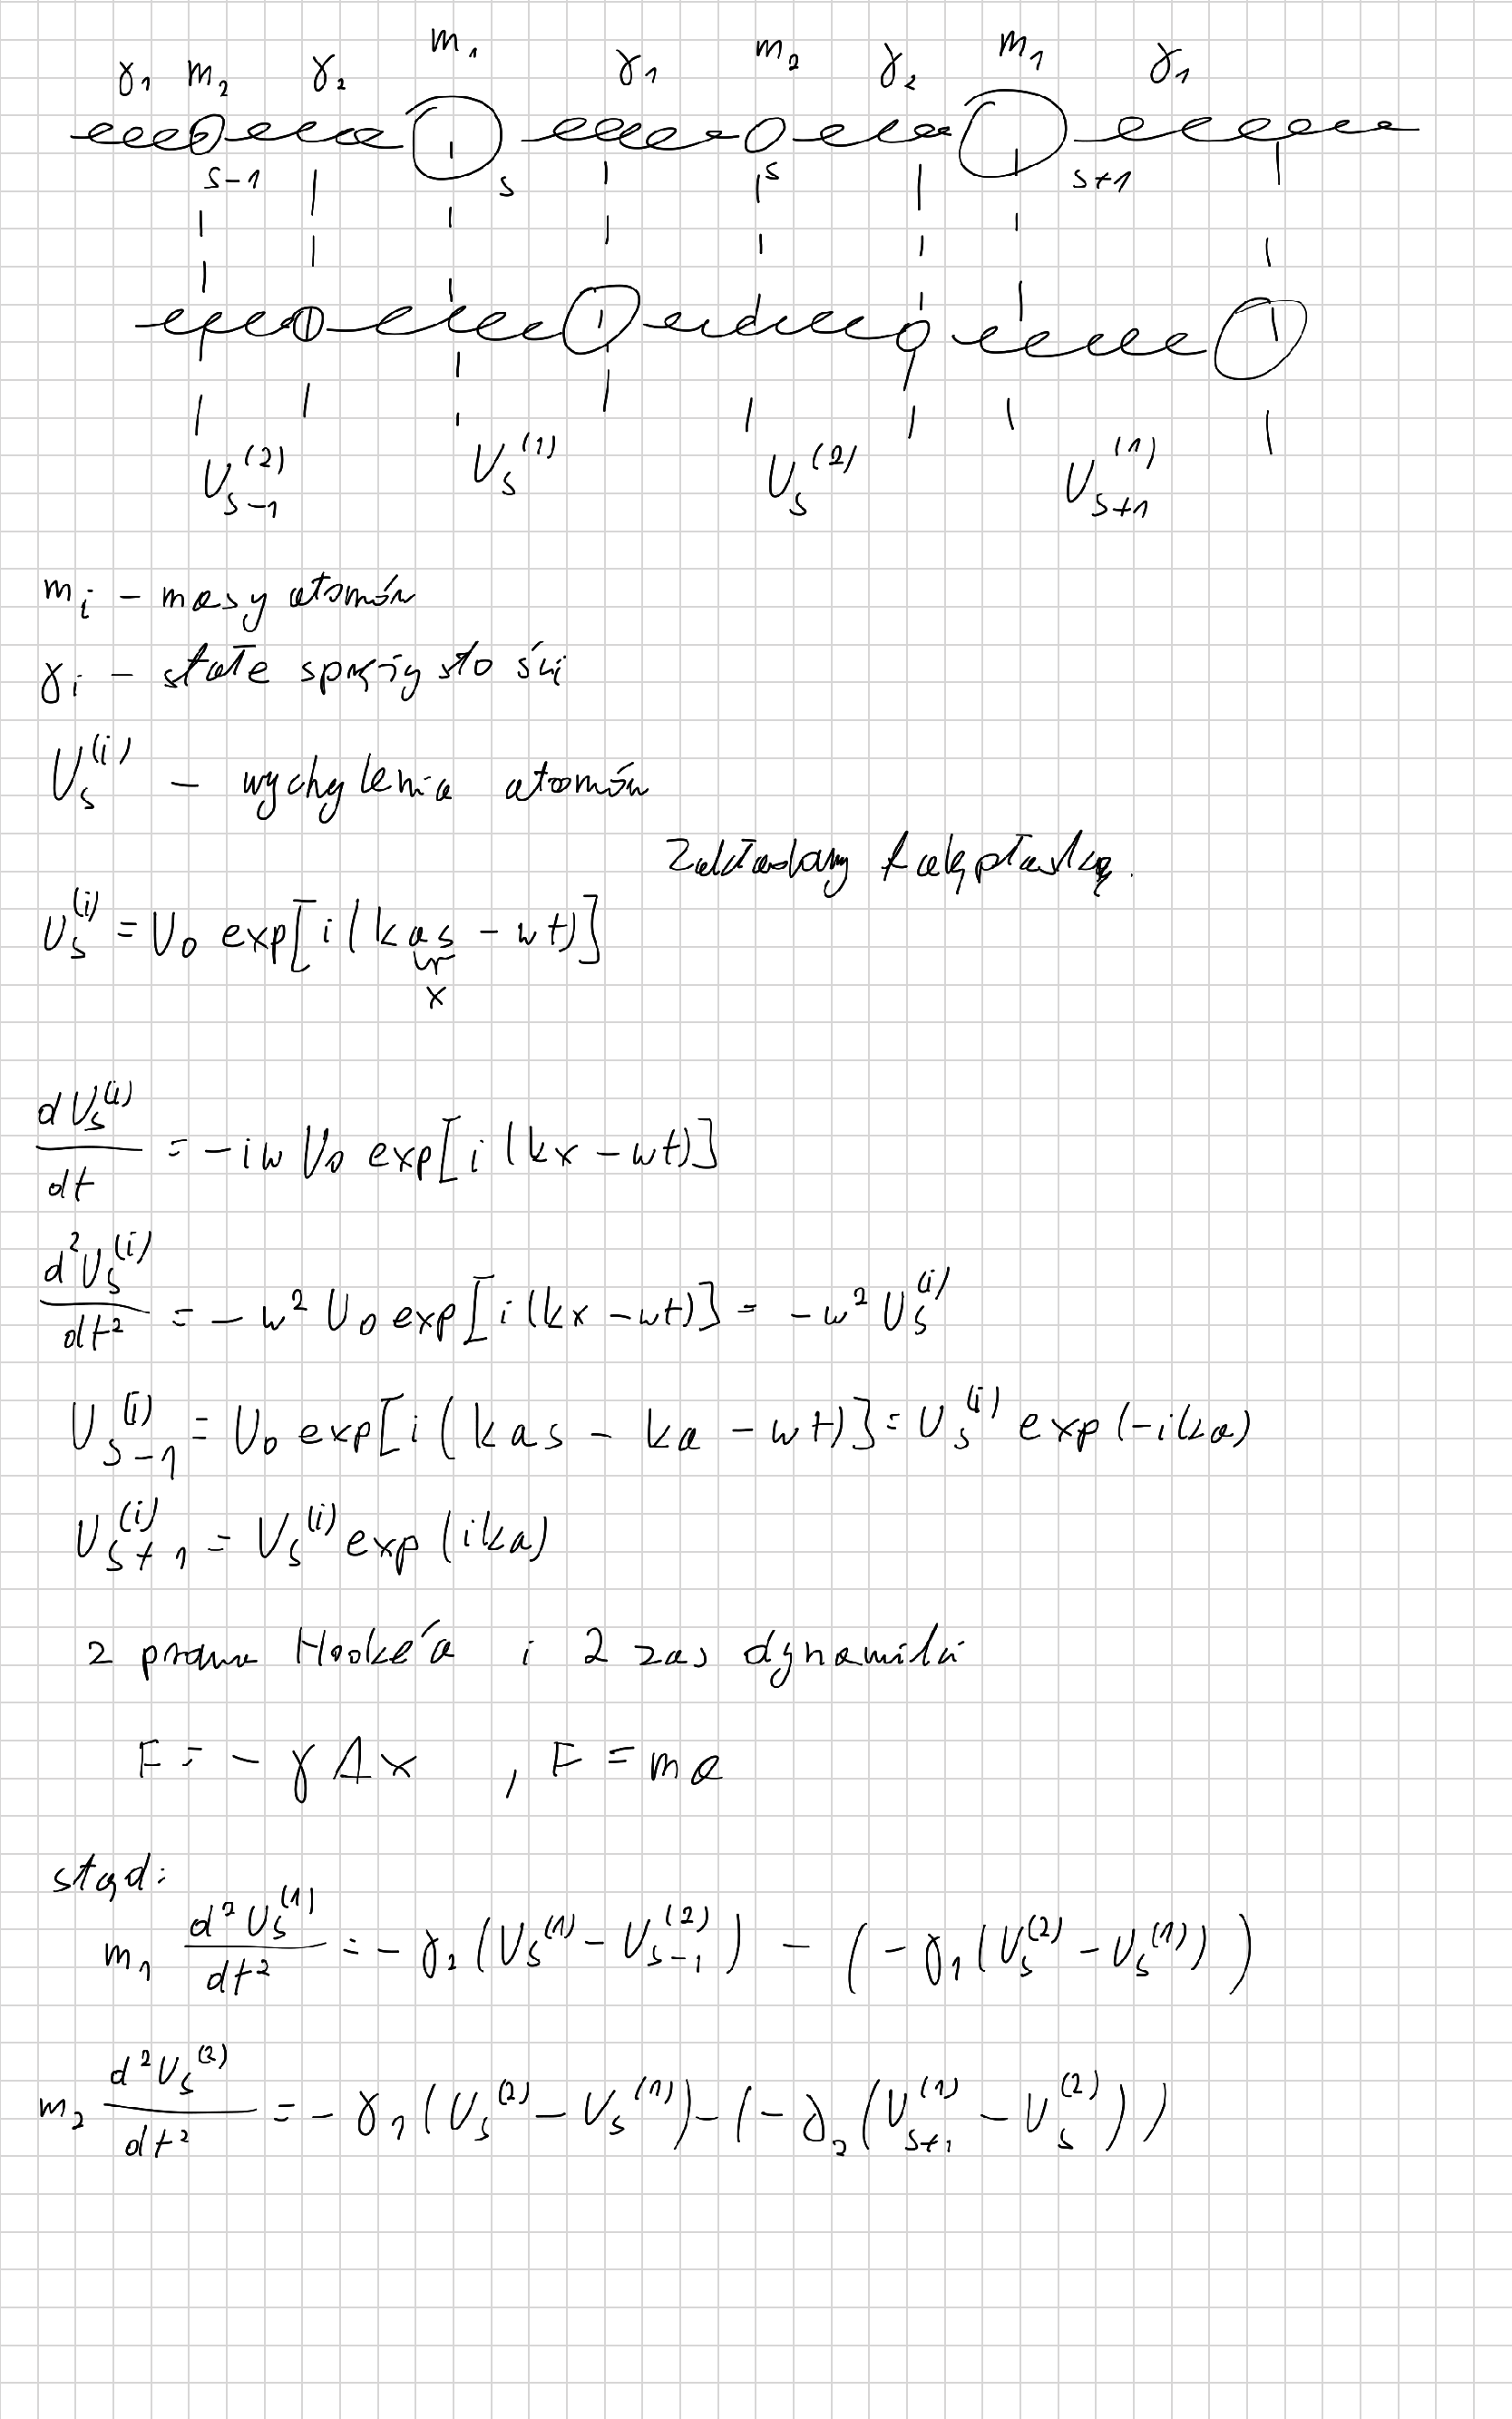
\includepdf[pages=-]{projekt2_zad1.pdf}

\section*{Zadanie 2 - nanostruktury półprzewodnikowe}
Projekt nanostruktury półprzewodnikowej opartej na studni kwantowej, która dzięki zjawisku elektroluminescencji emituje światło o długości $\lambda$ policzonej ze wzoru:

$$ \lambda = [\mbox{index (mod 6)} + 2] \cdot 100 + \mbox{index (mod 100)} = 230\mbox{ [nm] - światło nadfioletowe}$$

Ta długość fali odpowiada energii fotonu:

$$E_f = \frac{hc}{\lambda} = 5.39 eV$$

Założenia:
\begin{itemize}
	\item szerokość studni musi być nie mniejsza niż 5 krotność stałej sieciowej materiału
	\item różnica stałych sieci związków nie może przekraczać 10\% wartości maksymalnej
\end{itemize}

\begin{figure}[ht!]
    \centering
    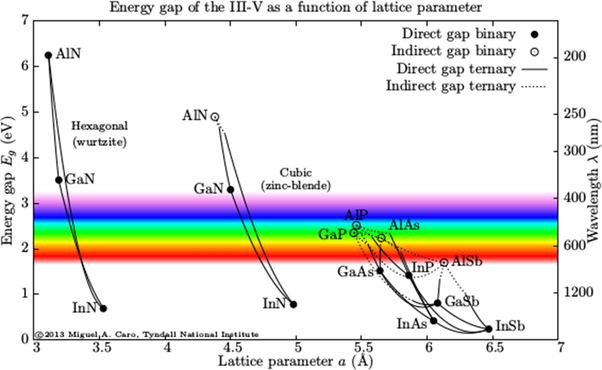
\includegraphics[width=0.7\textwidth]{./misc/polprzewodniki1.png}
    \centering
\end{figure}

\setcounter{figure}{0}
\renewcommand{\figurename}{Schemat}
\begin{figure}[ht!]
    \centering
    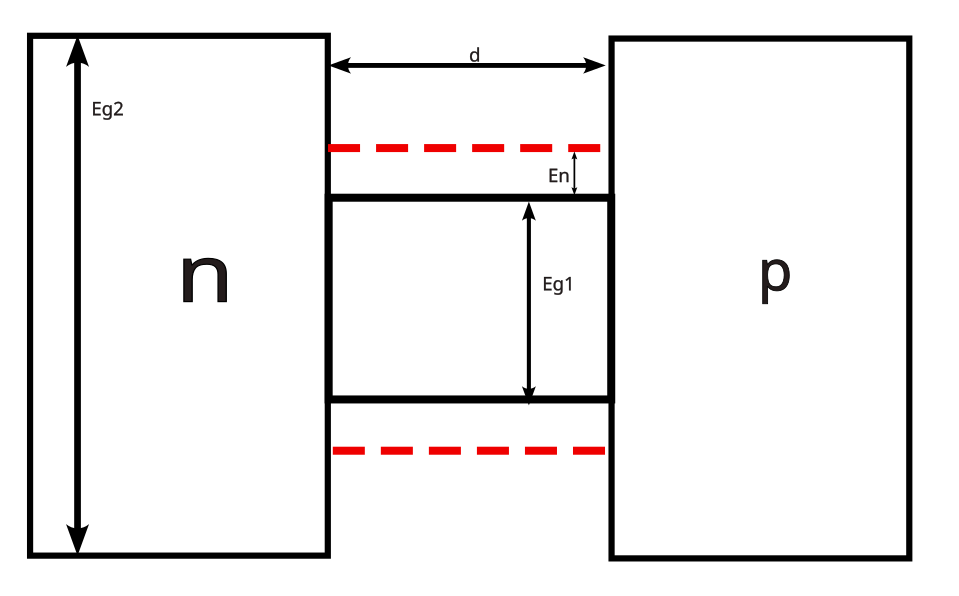
\includegraphics[width=0.7\textwidth]{./misc/scheme.png}
    \caption{Budowa nanostruktury}
    \centering
\end{figure}

\begin{itemize}
	\item $ E_n $ - poziom energetyczny studni (w tym zadaniu przyjmujemy n=1)
	\item $ E_{g1} $ - przerwa energetyczna studni
	\item $ E_{g2} $ - przerwa energetyczna okładek 
	\item $ d $ - szerokość studni 
\end{itemize}

Wiedząc, że:
\begin{equation}\label{En}
E_n = \frac{E_f - E_{g1}}{2}
\end{equation}
Szukamy na powyższym wykresie takiego materiału dla którego $E_{g1}<E_f$
Za materiał studni został wybrany związek $Al_{0.6}Ga{0.4}N$ w strukturze heksagonalnej
\begin{itemize}
	\item przerwa energetyczna $E_{g1}=5.3$ $eV$
	\item stała sieciowa $a_1=3.12$ \AA
\end{itemize}

Za materiał okładek został wybrany związek $AlN$ w strukturze heksagonalnej

\begin{itemize}
	\item przerwa energetyczna $E_{g2}=6.3$ $eV$
	\item stała sieciowa $a_2=3.10$ \AA
\end{itemize}

Proporcje związków i stałe sieciowe zostały wyznaczone metodą liczenia pikseli.

Wiedząc, że: 
\begin{equation}\label{en2}
E_n = \frac{h^2n^2}{8m_ed^2}
\end{equation}
oraz korzystając ze wzoru \ref{En}, możemy wyznaczyć szerokość studni d = 28.8 \AA.

Sprawdzając pierwsze założenie:
$$ \frac{d}{a_1} = 9.29 \approx 9 $$

Sprawdzając drugie założenie:
$$ \frac{\Delta a}{a_1} = 0.64 \% << 10\%$$ 


Wiedząc, że szerokość studni musi być wielokrotnościa wielkości atomu możemy podstawić d = 9a = 27.9\AA $ $ do wzoru \ref{en2}, a następnie ze wzoru \ref{En} wyznaczyć długość fali emitowanego przez zaprojektowany laser.
$$E_f = 5.4 eV \rightarrow \lambda = 229.7 nm $$



% zalozenia szerokosc minimum 5krotonosc stalej sieciowej (lattice) STUDNIA
% roznica stale sieciowej studni i okladek nie moze byc wieksza niz 10 % ich wartosci
\section*{Zadanie 3 - analiza termiczna}
Na podstawie danych z pliku $zad1_dta_1$ została wykreślona krzywa DSC:
\begin{figure}[H]
    \centering
    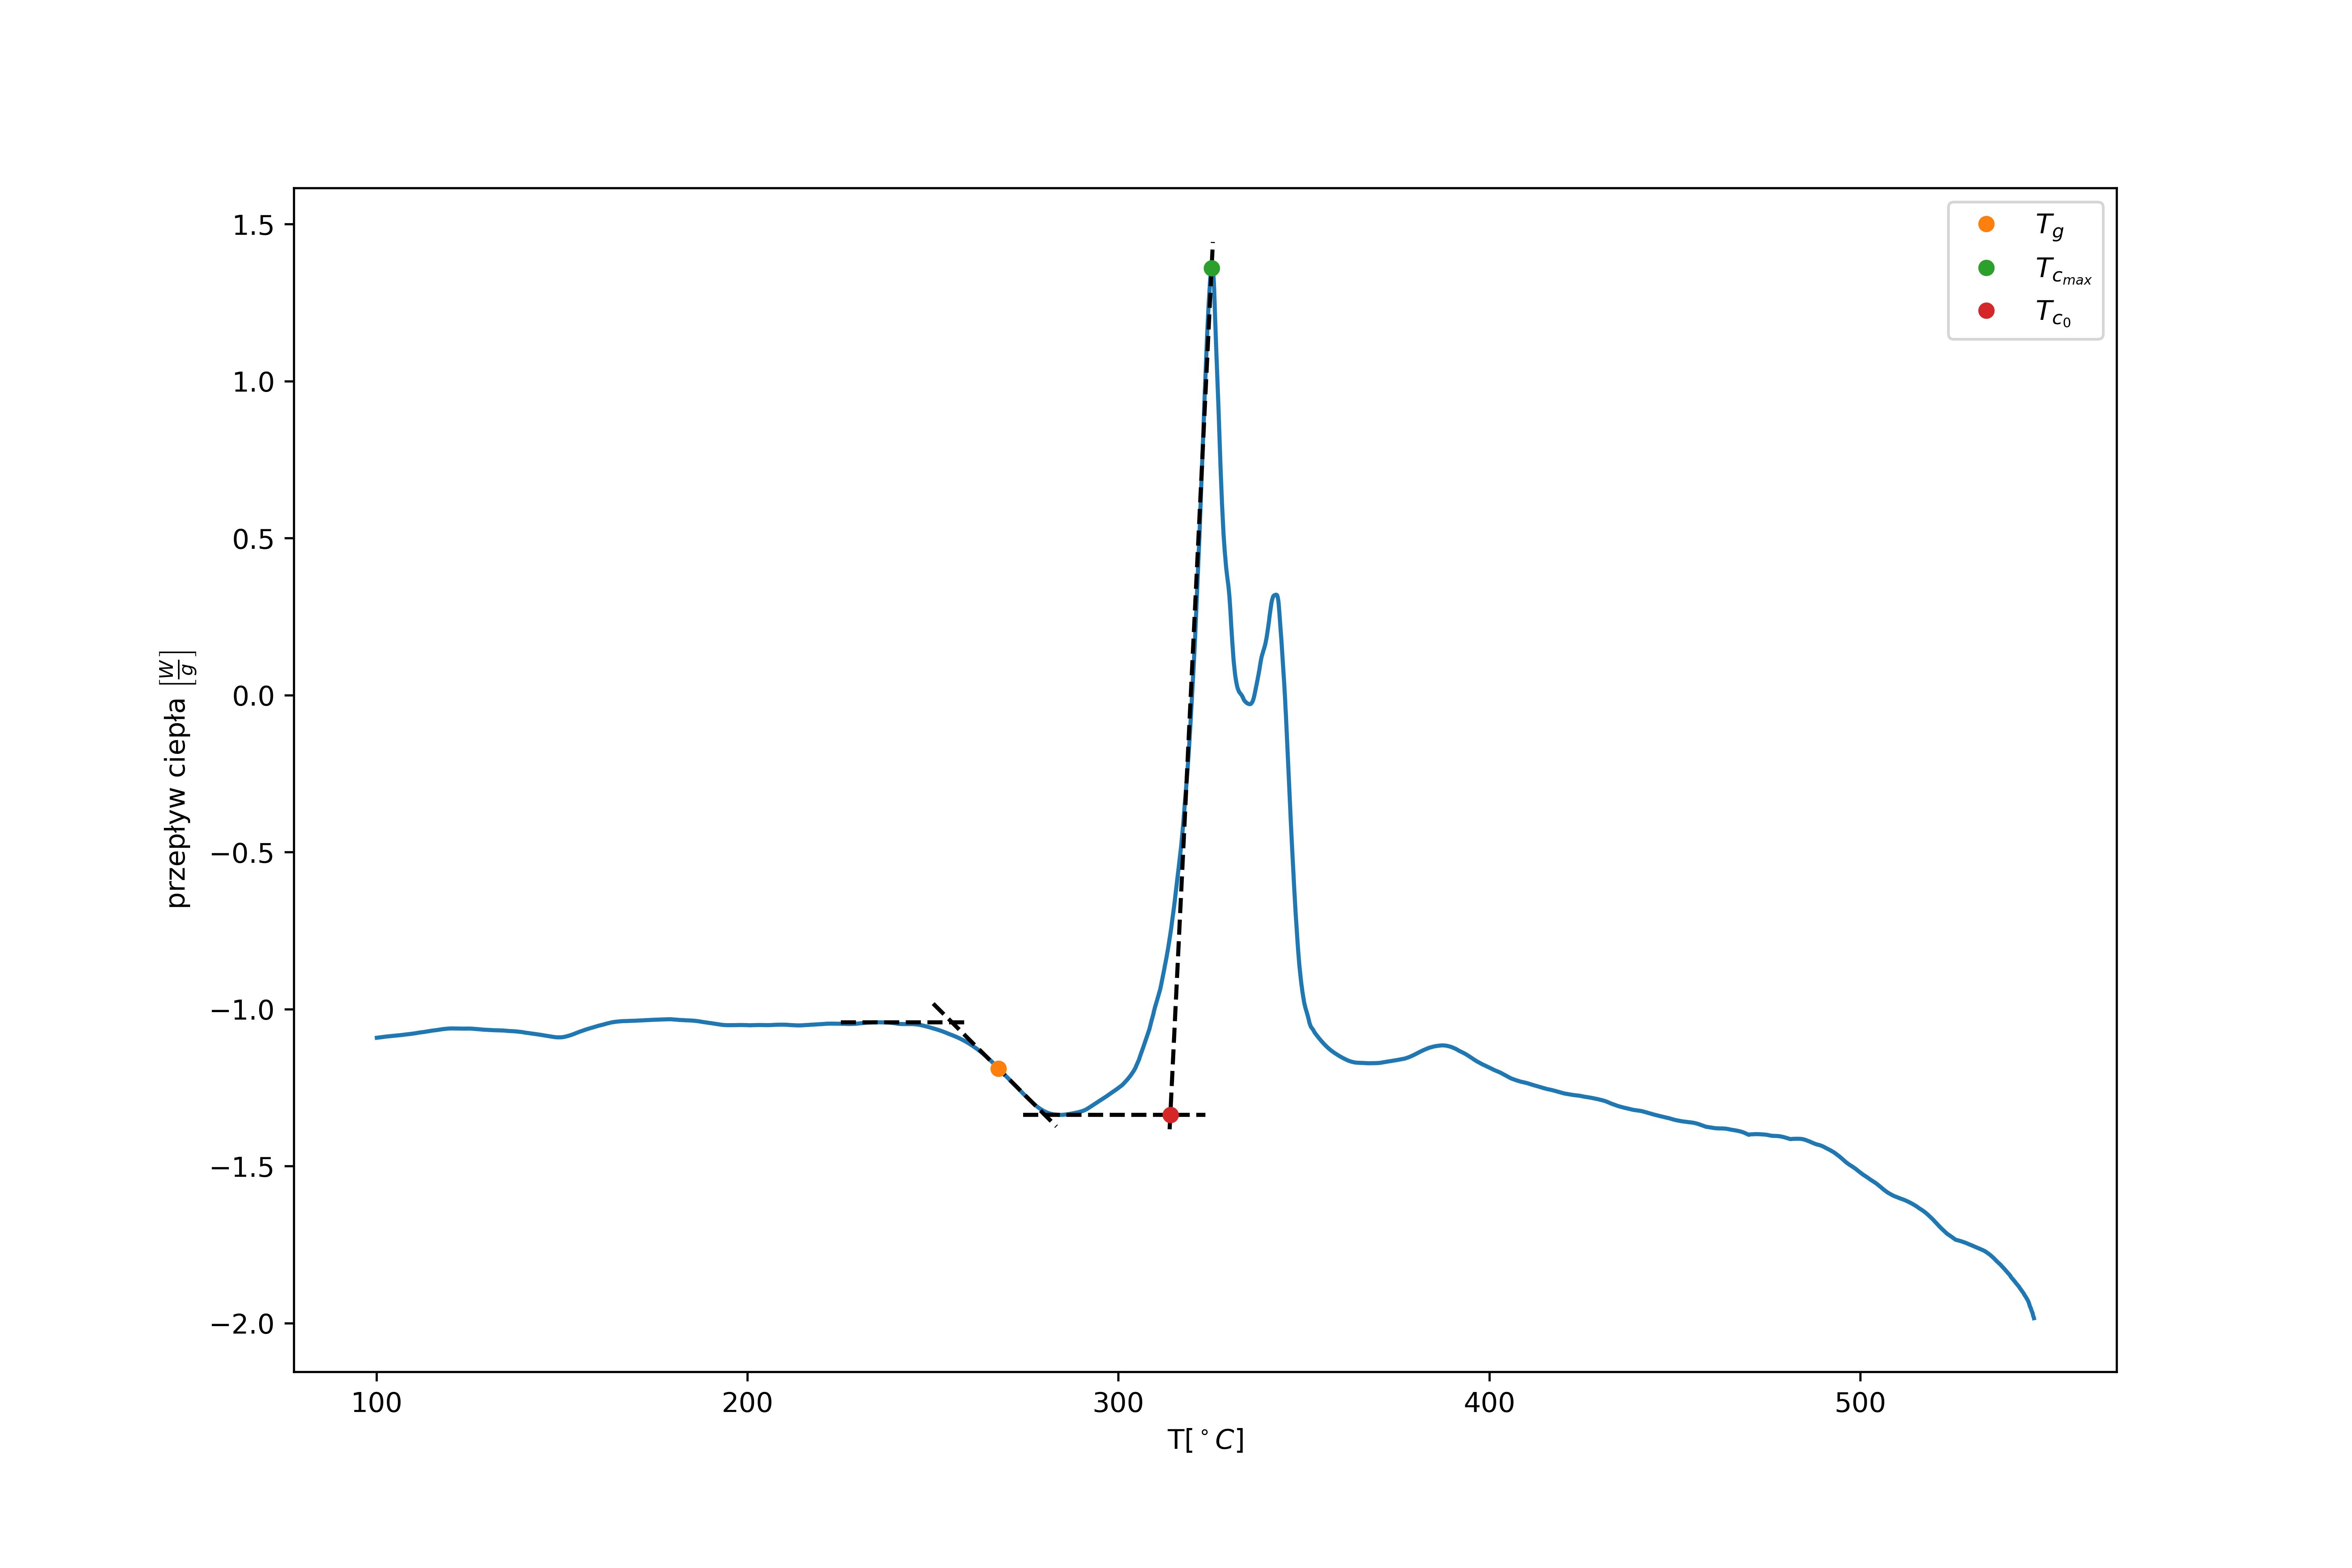
\includegraphics[width=0.7\textwidth]{zad3.jpg}
    \centering
\end{figure}
Dopasowując odpowiednie proste można odczytać temperatury:
\begin{itemize}
	\item $T_g$ - temperatura przjeścia szklistego wyznaczona jako środek odcinka nachylenia pierwszego spadku
	\item $T_{c_0}$ - temperatura początkowa krystalizacji wyznaczona jako przecięcie prostej horyzontalnej wychodzącej z minimum pierwszego spadku i prostej ekstrapolowanej z piku
	\item $T_{c_{max}}$ - temperatura maksymalna krystalizacji wyznaczona jako maksimum piku
\end{itemize}
Jak można zauważyć, na wykresie nie widnieje proces topnienia.
\end{document}
